Seguindo para as arquiteturas com poucos parâmetros treináveis, a primeira destas a ser treinada e testada foi a MobileNet. Para esta arquitetura, considerando ambas as abordagens, foi realizada mais uma vez uma busca em \emph{grid} de modelos utilizando os hiperparâmetros especificados anteriormente.

\begin{table}[h!]
\centering
\caption{Detalhamento dos melhores modelos obtidos com a arquitetura MobileNet para cada uma das abordagens consideradas neste trabalho.}
\label{tab:mobilenet}
\resizebox{\textwidth}{!}{\begin{tabular}{ccccccc}
\toprule
\textbf{Abordagem} & \textbf{Otimizador} & \textbf{\emph{Patience}}  & \textbf{Função de Ativação} & \textbf{Acurácia} & \textbf{F-Score} & \textbf{EER} \\
\midrule
Abordagem A & SGD & 15 & ReLU & $0.9606$ & $0.9318$ & $0.9304$ \\
Abordagem B & Adam & 15 & ReLU & $0.8856$ & $0.8658$ & $9.9475$\\
\bottomrule
\end{tabular}}
\end{table}

\begin{figure}[H]
\centering
\caption{Histórico de \emph{loss} e acurácia durante o treinamento dos melhores modelos obtidos com a arquitetura MobileNet.}
\label{fig:treinamento-mobilenet}
\subfloat[\emph{Loss} durante treinamento da melhor rede MobileNet para a abordagem A.\label{subfig:mobilenet-a-loss}]{%
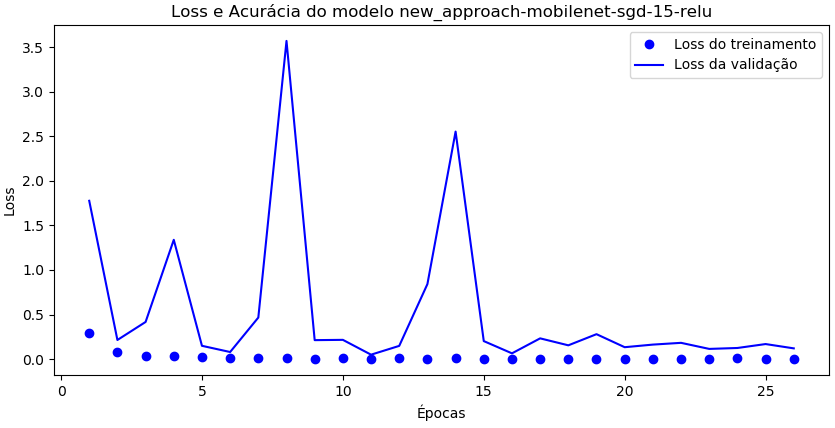
\includegraphics[width=0.47\textwidth]{imgs/mobilenet-a-loss}
}
\hfill
\subfloat[Acurácia durante treinamento da melhor rede MobileNet para a abordagem A.\label{subfig:mobilenet-a-acc}]{%
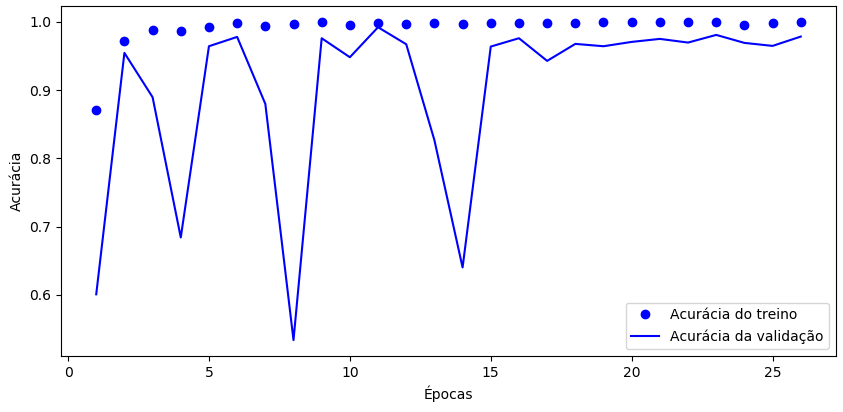
\includegraphics[width=0.47\textwidth]{imgs/mobilenet-a-acc}
}
\hfill
\subfloat[\emph{Loss} durante treinamento da melhor rede MobileNet para a abordagem B.\label{subfig:mobilenet-b-loss}]{%
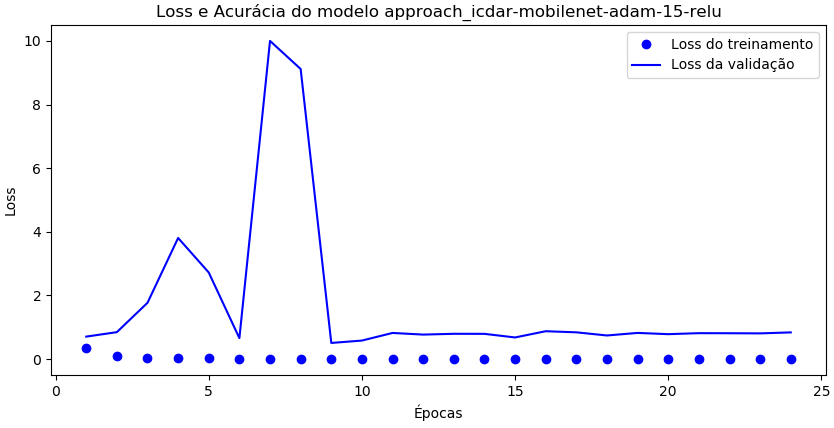
\includegraphics[width=0.47\textwidth]{imgs/mobilenet-b-loss}
}
\hfill
\subfloat[Acurácia durante treinamento da melhor rede MobileNet para a abordagem B.\label{subfig:mobilenet-b-acc}]{%
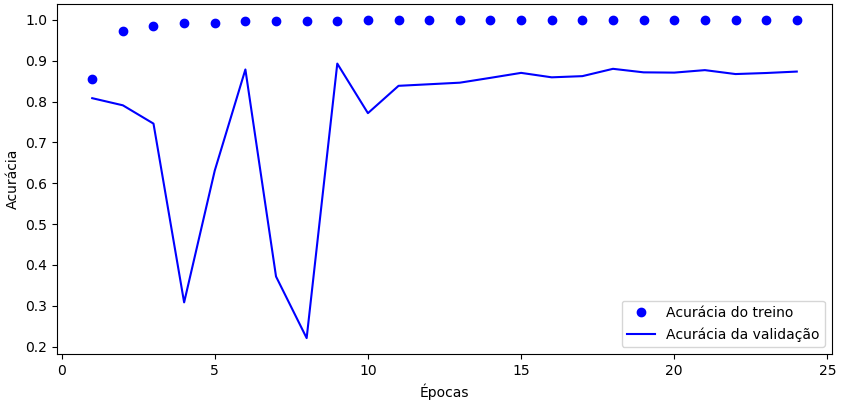
\includegraphics[width=0.47\textwidth]{imgs/mobilenet-b-acc}
}
\end{figure}

\begin{figure}[h]
	\centering
	\caption{Matrizes de confusão dos melhores modelos obtidos com a arquitetura MobileNet.}\label{fig:matrizes-mobilenet}
	\subfloat[Melhor MobileNet com a abordagem A\label{subfig:matriz-mobilenet-a}]{%
	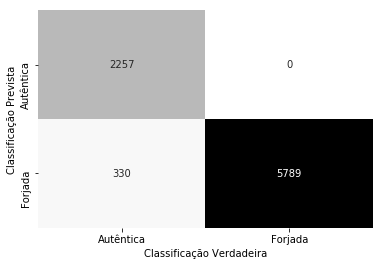
\includegraphics[width=0.47\textwidth]{imgs/matriz-mobilenet-a}
	}
	\hfill
	\subfloat[Melhor MobileNet com a abordagem B\label{subfig:matriz-mobilenet-b}]{%
	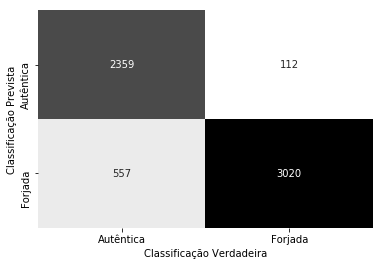
\includegraphics[width=0.47\textwidth]{imgs/matriz-mobilenet-b}
	}
\end{figure}